\appendix
\appendixpage
\addappheadtotoc
%
% \begin{figure}%[H]
%   \begin{center}
%   \includegraphics[width=0.8\textwidth]{}
%   \end{center}
%   \caption{Left panel shows data over the quake location, right panel shows data over the ribbon location. From top to bottom, plots show lightcurves from IRIS Si IV, Mg II, Balmer wavelengths and Mg II wing, with the bottom panel showing the lightcurve from SDO HMI.}\label{lcseries-bold}
% \end{figure}
\section{Ribbon Pixel Coordinates}\label{ribcoords}
%insert figure showing ribbon coords oplot
\begin{figure}%[H]
  \begin{center}
  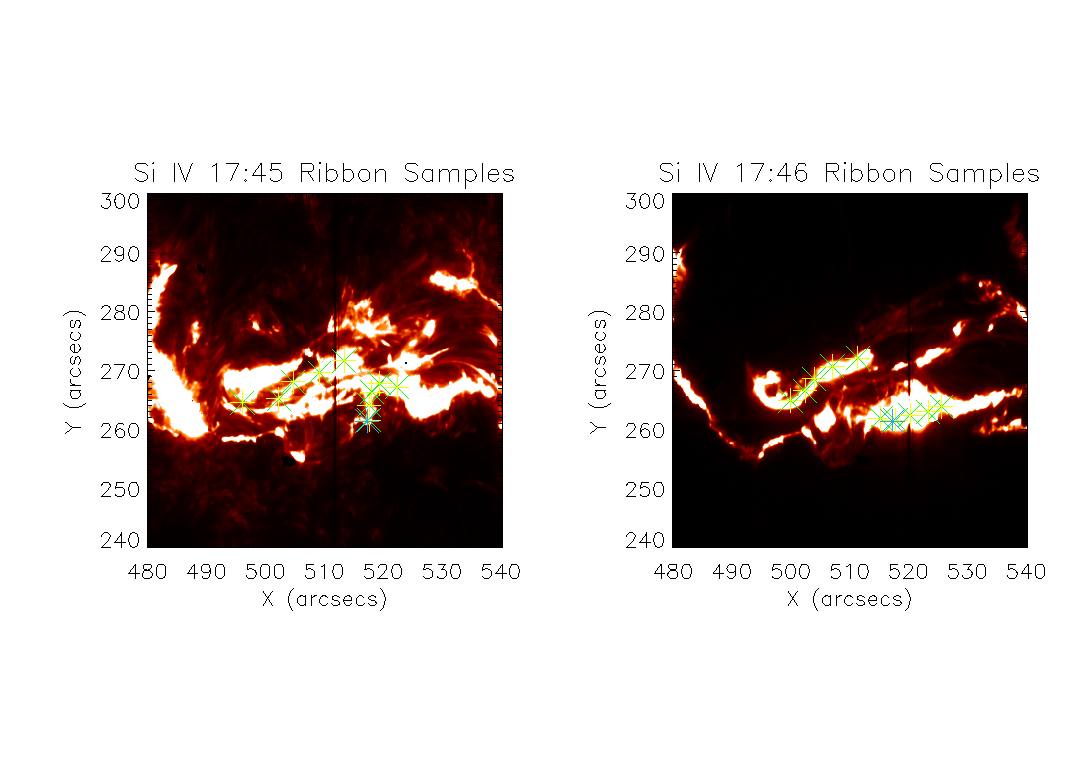
\includegraphics[width=0.8\textwidth]{29-Mar-14-SI-Ribbon-Coord-oplot}
  \end{center}
  \caption{Shows IRIS Si IV slit-jaw data with sampled ribbon and sunquake pixel coordinates marked in green and blue respectively. Twenty ribbon sample points are taken from two instances in time.}\label{sirib}
\end{figure}

\begin{figure}%[H]
  \begin{center}
  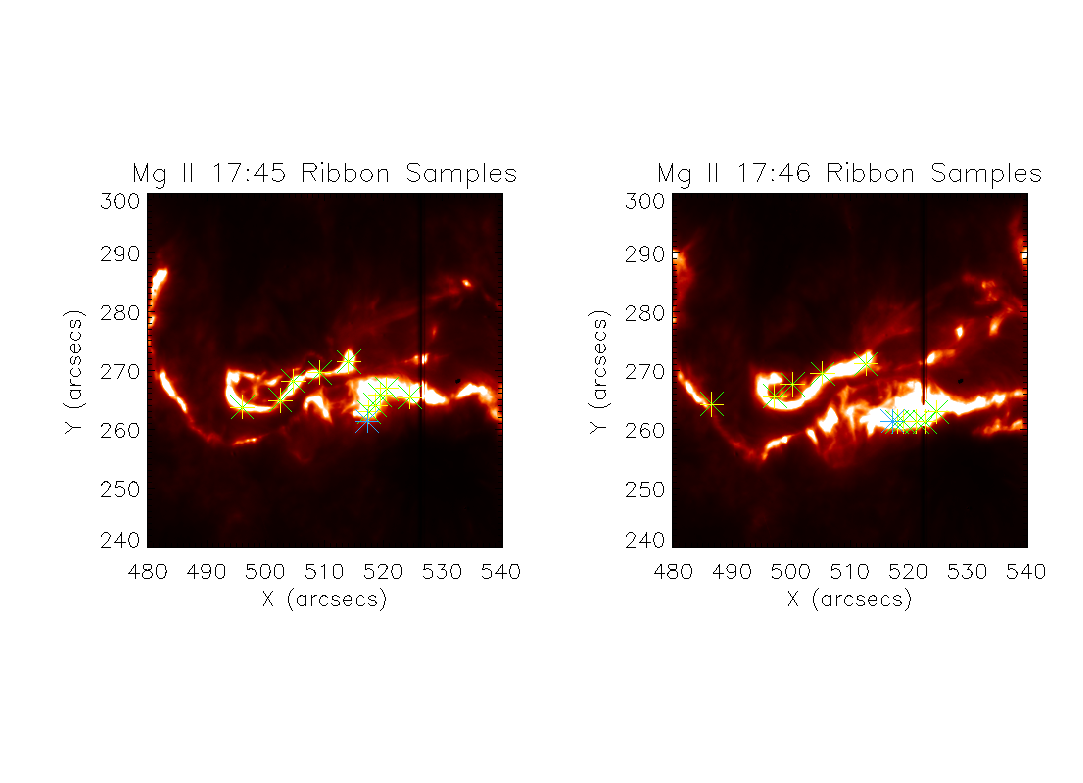
\includegraphics[width=0.8\textwidth]{29-Mar-14-MG-Ribbon-Coord-oplot}
  \end{center}
  \caption{Shows IRIS Mg II slit-jaw data with sampled ribbon and sunquake pixel coordinates marked in green and blue respectively. Twenty ribbon sample points are taken from two instances in time.}\label{mgrib}
\end{figure}

\begin{figure}%[H]
  \begin{center}
  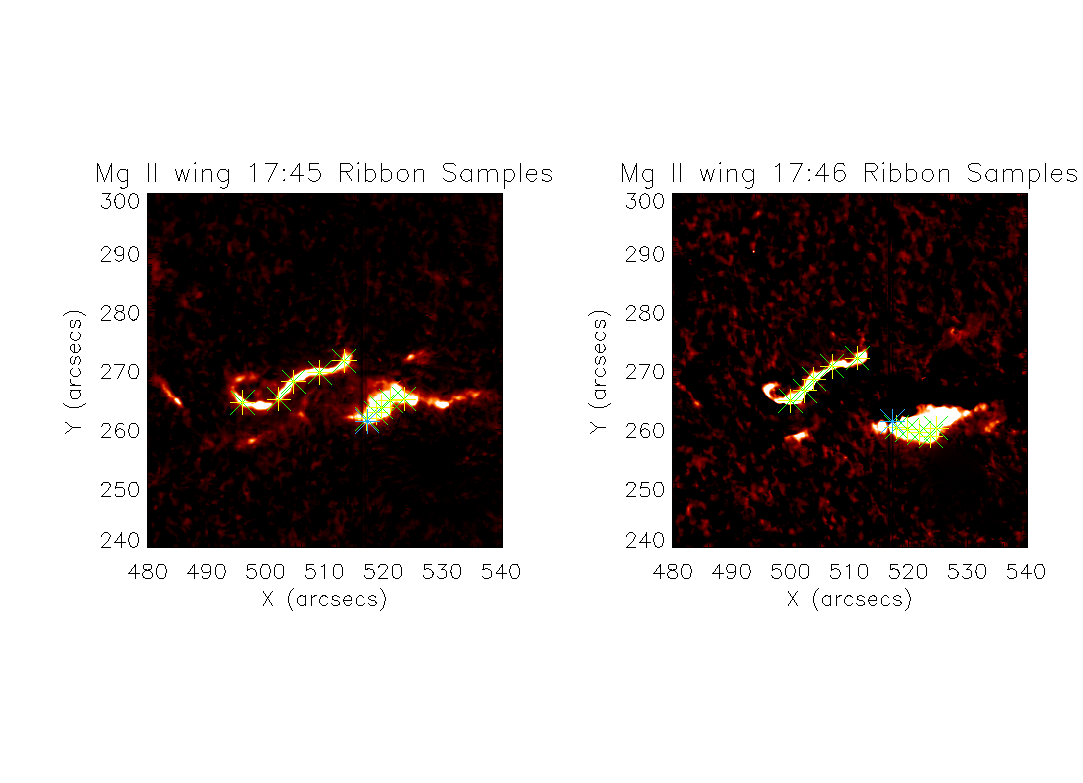
\includegraphics[width=0.8\textwidth]{29-Mar-14-MGW-Ribbon-Coord-oplot}
  \end{center}
  \caption{Shows IRIS Mg II wing slit-jaw data with sampled ribbon and sunquake pixel coordinates marked in green and blue respectively. Twenty ribbon sample points are taken from two instances in time.}\label{mgwrib}
\end{figure}
